\chapter{Evaluation and Results}

The reliability of the model has to be tested before incorporating it into the real world systems. If the accuracy of the model is below the desired value, then model is rejected. Otherwise we accept the model and proceed to deploy the system.

\section{Model evaluation}
Evaluating the model is to ensure that it produces reliable predictions which is significant. The model is built on a subset of data, which is called training data and they are applied to predict new data that are not part of this training subset. The model must be well balanced in terms of avoiding both over-fitting\footnote{Over-fitting is a problem where the evaluation of machine learning algorithms on training data is different from unseen data} and under-fitting\footnote{Under-fitting refers to a model that can neither performs well on the training data nor generalize to new data.}. The 80\%/20\% split of the dataset is generated for training and testing; thus here, 15 accidents are randomly selected for testing, and the remaining 56 are used for training the model. 

A two class prediction was selected in the case of fatal accidents in the stations to determine whether the accident happened during PM(0) or AM(1). Outcomes are labelled as either positive (PM) or negative (AM). The Model is tested on testing data (which is 20\% of the total data). A confusion matrix is built to analyse the accuracy of the model. The outcomes of the prediction are labelled as either positive or negative. If the prediction is positive and actual value is  also positive, then it is called a true positive (TP); with the same concepts, false positives(FP), true negatives(TN), and false negatives(FN) are realised. The four outcomes can be formulated as 2 x 2 confusion matrix as show in Figure \ref{fig:conf_mtx_m}. Accuracy is the ratio of the number of correct predictions over total predictions \cite{skiena_data_2017}. The best accuracy is 1.0, whereas the worst is 0.0. For this model, the accuracy is calculated using Equation \ref{eq:accuracy} and it is found to be 0.887 (or 88.7\%). Clearly, the model is more correct than incorrect when deciding whether the passengers involved in the accidents were there during the AM vs. PM

\begin{figure}
    \centering
    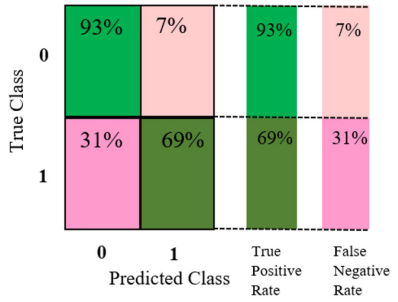
\includegraphics[scale=0.3]{chapters/images/conf_mtx_measured.png}
    \caption{Confusion matrix}
    \label{fig:conf_mtx_m}
\end{figure}

The area under the curve(AUC) was measured under the ROC\footnote{An ROC curve (receiver operating characteristic curve) is a graph showing the performance of a classification model at all classification thresholds \cite{roc}. The curve plots 2 parameters; true positive rate (TPR) and false positive rate(FPR) given by,  $$TPR = \frac{TP}{TP+FN}$$ $$FPR = \frac{FP}{FP+TN}$$} curve. The decision tree achieves higher AUC values of 0.90 which indicates an improved classifier performance (Figure \ref{fig:roc})

\begin{figure}
    \centering
    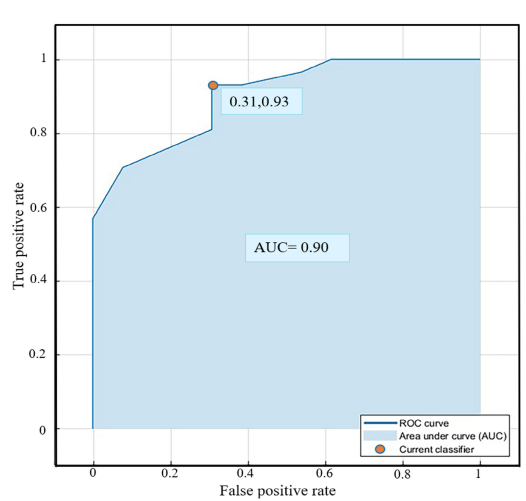
\includegraphics[scale=0.3]{chapters/images/roc.png}
    \caption{The ROC curve, which shows that AUC is 0.90. \cite{alawad_learning_2020}}
    \label{fig:roc}
\end{figure}

\section{Discussion}
New technologies like ML has a potential in suggesting safety improvements at railway stations. To train the ML model, a handful of accidents collected from RSSB reports are used. The accessibility to the data seems to be a big challenge, because of the privacy concerns poor data collection system. For the purpose of extracting the most helpful data, we must integrate some of the systems in the railway stations and perhaps automate data collection.

For the purpose of this project, 71 incidents are studied. This volume is quite low for a data science project. But model trained from this dataset has shown an acceptable performance. Model needs to be tested on more data to ensure its suitability. It is noted that the platform is a significant area of the station where many accidents occur. Some factors are obvious, such as time, where PM saw more accidents than AM. A high ratio of accidents occurring for males has been seen in two important age groups: the young and the old. 

Weather conditions, building design, the number of people present at the station at the time of the incident, and other variables may also have an impact on the causes of accidents. But in this work such factors are not considered. 
The DT method has been applied, and it shows how the prediction path predicts the target instances. The results need to further verified as data availability increases and with more sophisticated tools because of the challenges mentioned above. Some of the objectives of the current model are;
\begin{enumerate}
    \item Providing information that future railway stations may demand through In depth analysis and classification.
    \item  identifying any potential gaps in the current safety frameworks or processes, and then strengthening the system through advanced technology.
    \item Prediction of risk or consequences based on recorded safety data.  
\end{enumerate}

ML is a promising technology that can learn from historical data and overcome the uncertainty associated with traditional approach. In future, this model can be extended to integrate many systems to make intelligent decisions in real time. The emerging technologies like cloud computing, IoT etc can fuel the development in this direction. Additionally, the information produced by sophisticated analytical tools improves understanding of the current situation and may be useful for developing new stations.

